\documentclass[a4paper,11pt]{article}
\usepackage[utf8]{inputenc}
\usepackage[spanish]{babel}
\usepackage{cite}
\usepackage{apalike}
\bibliographystyle{apalike}
\usepackage[pdftex]{graphicx}
\usepackage{hyperref}

\begin{document}
\title{Producción de Biogás a partir de residuos}
\author{Julia Rivera Jiménez}
\date{20-12-2020}
\maketitle

{\em Resumen:} \\ 
URL del repositorio: \url{https://github.com/julia030798/proyecto_final} \\
El objetivo de este trabajo es proporcionar una visión general de la producción de biogás a partir de residuos lignocelulósicos ya que la demanda mundial de energía es alta y la mayor parte de esta energía se produce a partir de recursos fósiles. El uso irracional actual de combustibles fósiles y el impacto de los gases de efecto invernadero en el medio ambiente están impulsando la investigación sobre la producción de energía renovable a partir de recursos orgánicos y desechos. Estudios recientes informan que la digestión anaeróbica (DA) es una tecnología alternativa eficiente que combina la producción de biocombustible con la gestión sostenible de residuos.
\\\\
{\em Palabras clave:}
biogás, residuos lignocelulósicos, energía renovable, digestión anaeróbica (DA), biocombustible, sostenible.

\section{Introducción}
Los escenarios han demostrado que la demanda de energía aumentará durante este siglo en un factor de dos o tres, como resultado del crecimiento de la población y el consumo de energía per cápita. Al mismo tiempo, las concentraciones de gases de efecto invernadero (GEI) en la atmósfera están aumentando rápidamente, siendo las emisiones de $CO_{2}$ derivadas de combustibles fósiles el contribuyente más importante. Las estadísticas indican que los tipos más comunes de combustibles fósiles utilizados en la actualidad son el petróleo y sus productos, el gas natural y el carbón.
\\\\
Para minimizar los impactos relacionados con el calentamiento global y el cambio climático, las emisiones de GEI deben reducirse a menos de la mitad de los niveles de emisiones globales de 1990. Otro desafío global importante es la seguridad del suministro de energía, porque la mayoría de las reservas convencionales de petróleo y gas conocidas son concentrado en regiones políticamente inestables \cite{Weiland2010}. 
\\\\
Se estima que en términos de fuente primaria utilizada, para 2030, la estructura de producción de energía se basará en: 75-85\% de combustión de combustible convencional, 10-20\% de fisión nuclear, 3-5\% de energía hidráulica, aprox. 3\% de la energía solar y eólica \cite{Popescu2010}.
\\\\
Se ha reconocido la importancia de los recursos de biomasa y se han incrementado enormemente en el marco de los sistemas energéticos. Esto no solo se basa en el desarrollo actual del crecimiento de la conciencia ambiental pública y su apariencia exterior, sino también en el hecho de que la energía de la biomasa es la única energía renovable que logra una potencia continua, como resultado de la planificación y el almacenamiento del recurso energético disponible \cite{Koenig2008}.
\\\\
La bioenergía a partir de recursos renovables ya es una alternativa viable a los combustibles fósiles; sin embargo, para satisfacer la creciente necesidad de bioenergía, se deben considerar varias materias primas. La lignocelulosa es el material orgánico más abundante en la tierra, en diversas cantidades, calidades y formas, por lo que es una materia prima prometedora para la producción de bioenergía \cite{Petersson2007}.
\\\\
La digestión anaeróbica y la producción de biogás son medios prometedores para lograr múltiples beneficios ambientales y producir un vector energético a partir de recursos renovables. La sustitución de los combustibles fósiles por biogás normalmente reduce la emisión no solo de gases de efecto invernadero, sino también de óxidos de nitrógeno y azufre, hidrocarburos y partículas \cite{Boerjesson2006}.

\subsection{Estado del arte de la producción de biogás}
La producción de biogás mediante DA es la forma más sencilla de extraer energía de los materiales de desecho, pero está asociada y afectada por múltiples factores. En las últimas décadas, se han innovado muchas tecnologías de pre- y pos- proceso de producción de biogás para lograr la máxima producción de biogás. Esto puede incluir el pretratamiento, microorganismos, control y monitoreo de procesos, codigestión, separación de fases, Biorreactores de membrana anaeróbica (AnMBRs) y purificación de biogás \cite{Maurya2019}.
\\\\
Las técnicas avanzadas, como la separación de hidratos, la separación criogénica, los métodos biológicos, el enriquecimiento de membranas, la mejora in situ, la digestión anaeróbica multietapa y de alta presión, representan los avances modernos en las técnicas de mejora del biogás. La mayoría de los países están en proceso de promulgar leyes para regular la industria del biogás \cite{Korbag2020}.
\\\\
Sin embargo, estas tecnologías deben integrarse entre sí de tal manera que mejoren la generación de biogás con un enfoque económico y sostenible. 

\section{Digestión anaeróbica}
La digestión anaeróbica consiste en una serie de procesos en los que los microorganismos descomponen material biodegradable en ausencia de oxígeno, utilizado con fines industriales o domésticos para gestionar residuos y/o liberar energía. Se usa ampliamente como parte del proceso para tratar aguas residuales. Como parte de un sistema integrado de gestión de residuos, la digestión anaeróbica reduce la emisión de gases de vertedero a la atmósfera. 

\begin{table}[h]
\centering
\begin{tabular}{|p{6cm}|p{6cm}|}
\hline
{\bf Etapa} & {\bf Reacción} \\
\hline
Acidogénesis & $C_{6}H_{12}O_{6}$ + $H_{2}O$ $\longrightarrow$ $2CH_{3}COO^-$ + $2CO2$+ $2H^+$ + $4H_{2}$ \\
\hline
Acetogénesis & $CH_{3}CH_{2}COO^-$  + $3H_{2}O$ $\longrightarrow$ $CH_{3}COO^-$ + $HCO_{3}^-$ + $H^+$ + $3H_{2}$ \\
\hline
Metanogénesis &  $4H_{2}$ + $\frac{1}{4}$ $HCO_{3}^-$ + $\frac{1}{4}$ $H^+$ $\longrightarrow$ $\frac{1}{4}$ $CH_{4}$ + $\frac{3}{4}$ $H_{2}O$ \\
\hline
\end{tabular}
\caption{Reacciones en la degradación anaeróbica \cite{Moraes2015}}
\label{Tabla 1}
\end{table}

La digestión anaeróbica se usa ampliamente como fuente de energía renovable porque el proceso produce un biogás rico en metano y dióxido de carbono adecuado para la producción de energía, lo que ayuda a reemplazar los combustibles fósiles. El digestato rico en nutrientes que también se produce se puede utilizar como fertilizante. El proceso de digestión comienza con la hidrólisis bacteriana de los materiales de entrada para descomponer los polímeros orgánicos insolubles, como los carbohidratos, y ponerlos a disposición de otras bacterias. Las bacterias acidógenas luego convierten los azúcares y aminoácidos en dióxido de carbono, hidrógeno, amoníaco y ácidos orgánicos. 
\\\\
Las bacterias acetogénicas luego convierten estos ácidos orgánicos resultantes en ácido acético, junto con amoníaco, hidrógeno y dióxido de carbono adicionales. Finalmente, los metanógenos convierten estos productos en metano y dióxido de carbono. La experiencia técnica requerida para mantener digestores anaeróbicos a escala industrial, junto con los altos costos de capital y la baja eficiencia del proceso, habían limitado el nivel de su aplicación industrial como tecnología de tratamiento de desechos \cite{Ionel2010}.

\section{Biodigestores}
Los biodigestores son sistemas diseñados para optimizar la producción de biogás a partir de desechos agrícolas, estiércol o efluentes industriales, entre otros, los cuales permiten así la obtención de energía limpia y de bajo costo a partir de una fuente renovable \cite{RivasSolano2010}.
\\
\begin{figure}[h]
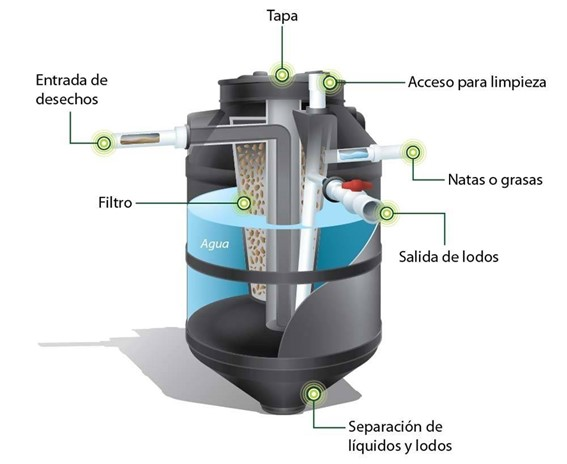
\includegraphics[scale=.75]{ImagenBiodigestor}
\caption{Esquema de un biodigestor \cite{Autores2013}}
\label{Figura 1}
\end{figure}
\\
Uno de los parámetros matemáticos que permite estimar la producción de biogás en un biodigestor es la productividad de metano o productividad metanoica, la cual se define como la cantidad de metano generado en la unidad de tiempo con respecto a la materia dispuesta en el reactor. 
\\\\
De esta manera, la expresión matemática que permite calcular la productividad de metano de un determinado resto orgánico en un tiempo dado, es la siguiente \cite{Sogari2003}:

\begin{displaymath}
P_{CH_{4}}=\frac{V_{CH_{4}}}{V_{reactor}*t}
\end{displaymath}

Donde $V_{CH_{4}}$ es el volumen de metano generado; $V_{reactor}$ es el volumen de materia dispuesta en el recinto fermentador y t es el tiempo considerado \cite{Sogari2003}.

\bibliographystyle{apalike}
\bibliography{Biblio}
\end{document}
